\section{Funções Vetoriais e Limites}

\begin{definb}{}{}
Uma \dt{função vetorial} é uma função cujo domínio é um conjunto de números reais e cuja imagem é um conjunto de vetores em $\R^n$, denotada por:
\[\begin{array}{lcl}
\vec{r}: & D\subset \R &  \longrightarrow \R^n\\
         & t           & \longmapsto \vec{r}(t)=(f_1(t),f_2(t),\ldots,f_n(t)).
\end{array}\]

As funções $f_1,\ldots,f_n$ são chamada \dt{funções componentes}.
\end{definb}

\begin{exeb}{}{}
\begin{enumerate}
\item $\vec{r}(t)=(t,t)$, $t\in \R$.
\item $\vec{r}(t)=(t,1,0)$, $t\geq 0$.
\end{enumerate}
\end{exeb}
\newpage


\marcador{subsection}{Limite e Continuidade}

\begin{definb}{}{}
Sejam $\vec{r}(t)=(f_1(t),f_2(t),\ldots,f_n(t))$ uma função vetorial com domínio $D$. Definimos o \dt{limite de $\vec{r}(t)$ quanto $t$ tende a $a\in D$} por
\[\lim\limits_{t\to a}\vec{r}(t)=\left(\lim\limits_{t\to a}f_1(t),\ldots,\lim\limits_{t\to a}f_n(t)\right), \]
desde que o limite das funções componentes existam.
\end{definb}

\begin{exerb}{}{}
Determine $\lim\limits_{t\to 0}\vec{r}(t)$, onde $\vec{r}(t)=(1+t^3, te^{-t})$.
\end{exerb}
\vspace{5cm}


\begin{definb}{}{}
Uma função vetorial $\vec{r}$ é \dt{contínua em $a$} se $\lim\limits_{t\to a}\vec{r}(t)=\vec{r}(a)$.
\end{definb}
Em vista desta definição, uma função $\vec{r}$ é {\color{blue}contínua em $a$} se, e somente se, cada uma de suas {\color{blue}componentes é contínua em $a$}.


\newpage



\marcador{subsection}{Curvas Parametrizadas}

Quando uma função vetorial \dt{$\vec{r}(t)=(f(t),g(t))$}, está definida em um intervalo $I$ da reta e  é \dt{contínua}, então o conjunto {\color{red}$C$} de todos os pontos $(x,y)$ do plano tais que
\begin{equation}\label{parametricas}
x={\color{blue}f(t)}\ \text{ e } y={\color{blue}g(t)}
\end{equation}
quando $t$ varia formam uma {\color{red}curva no plano}. As equações em  {\color{red} \eqref{parametricas}} são ditas {\color{red} equações paramétricas de $C$}, \dt{\(\vec{r}\)} é dita ser uma {\color{red}parametrização de $C$} e $t$ é chamado de  {\color{red} Parâmetro}.
\begin{exeb}{}{}
Determine as curvas parametrizadas por:
\begin{enumerate}
\item $\vec{r}(t)=(\cos(t),\sin(t))$, $t\in [0,2\pi]$.
\item $\vec{r}(t)=(\cos(2t),\sin(2t))$, $t\in [0,2\pi]$.

\end{enumerate}
\end{exeb}
\blfootnote{
Veja como plotar curvas parametrizadas usando Python \href{https://reginaldodr.github.io/academic/posts/curvas-parametricas/curvas-parametricas.html}{Curvas parametrizadas com Python}
}

\newpage


\begin{caixaazul}{Parametrização do Gráfico de uma Função}
O gráfico de qualquer função ${\color{blue}y=f(x)}, x\in I\subset\R$, pode ser parametrizado de forma natural usando a variável {\color{red}$x$ como parâmetro}, da seguinte forma:
\[\vec{r}({\color{red}t})=({\color{red}t},{\color{blue}f(t)}),\ {\color{red}t\in I}.\]
\end{caixaazul}

\begin{exeb}{}{}
 Determine uma parametrização para as curvas:
\begin{enumerate}[(a)]
\item A parábola $y=x^2$.
\item O gráfico da função \(y=\cos(x)\).
\item \(e^y-x^2=1\).
\item \(x=y^2+y\)
\end{enumerate}
\end{exeb}
\newpage




Se em uma equação polar {\color{blue}a coordenada $r$ estiver em função de $\theta$}, isto é, {\color{blue}$r=f(\theta)$}, então podemos usar {\color{red}$\theta$ como parâmetro} e parametrizar a curva representada pela equação polar da seguinte forma:

\begin{center}
\destaque{
\(
\vec{\alpha}({\color{red}\theta})=f({\color{red}\theta})(\cos {\color{red}\theta},\sin {\color{red}\theta})
\)
}
\end{center}

\begin{exeb}{}{}
Determine uma parametrização para a  cardioide $r=1+\cos \theta$
%\[\vec{\alpha}(\theta)=(r\cos \theta,r\sin \theta)=(1+\cos (\theta))(\cos \theta,\sin \theta),\ \theta\in [0,2\pi].\]

\end{exeb}



\vfill
\begin{casab}{}{}
\begin{enumerate}
\item  Determine uma parametrização para o segmento de reta que entre os pontos $(1,0)$ e $(2,5)$.
\item Determine a curva parametrizada por $\vec{r}(t)=(2\cos(t),\sin(t))$, $t\in [0,2\pi]$.
\item		Esboce a curva que é representada pelas equações polares abaixo.
\begin{enumerate}
\item $r=2\cos\theta$

\item $r=\cos 2\theta$ (rosácea de quatro pétalas)
\end{enumerate}
\end{enumerate}
\end{casab}
\newpage


\marcador{subsection}{Curvas Parametrizadas no Espaço}

Quando uma função vetorial {\color{blue}$\vec{r}(t)=(f(t),g(t),h(t))$}, está definida em um intervalo $I$ da reta e  é \dt{contínua}, então o conjunto {\color{red}$C$} de todos os pontos $(x,y,z)$ do plano tais que
\begin{equation}\label{parametricas2}
x={\color{blue}f(t)},\  y={\color{blue}g(t)}\ \text{ e } z={\color{blue}h(t)}
\end{equation}
quando $t$ varia formam uma {\color{red}curva no espaço}. As equações em  {\color{red} \eqref{parametricas2}} são ditas {\color{red} equações paramétricas de $C$}, ${\color{blue}\vec{r}}$ é dita ser uma {\color{red}parametrização de $C$} e $t$ é chamado de  {\color{red} Parâmetro}.

\begin{center}
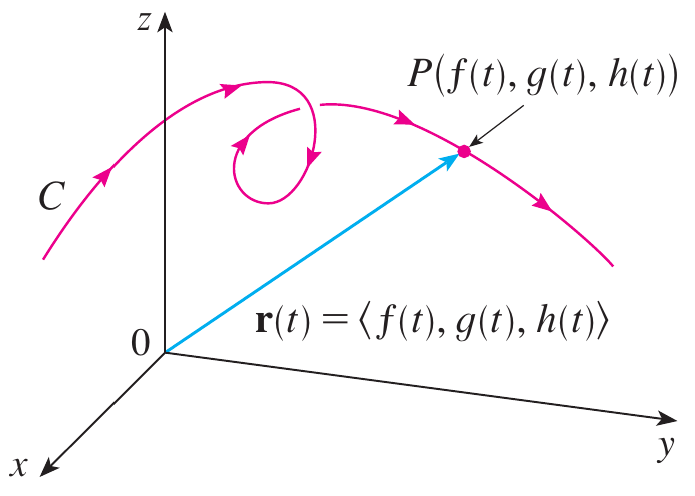
\includegraphics[scale=.5]{figuras/curvas/param-curvas-espaco.png}
\end{center}


\begin{exeb}{}{}
Determine as curvas parametrizadas por:
\begin{enumerate}
\item $\vec{r}(t)=(1,t,2t)$, $t\in (0,1)$.
\item $\vec{r}(t)=(\cos(t),\sin(t),t)$, $t\in [0,2\pi]$.
\end{enumerate}
\end{exeb}
\newpage


\begin{caixaazul}{Hélices}
A curva do exemplo anterior é uma \dt{hélice}. Existem vários tipos de hélices, as mais simples são as \dt{hélices circulares com passo constante}, cuja  parametrização e dada por
\[\vec{r}(t)=({\color{red}a}\cos(t),{\color{red}a}\sin(t),{\color{blue}b}t),\]
onde ${\color{red}a},{\color{blue}b}$ são constantes.

As hélices aparecem em diversas aplicações, como por exemplo no formato de molas e no modelo de DNA que é formado por uma dupla hélice.
\end{caixaazul}
\bigskip

\begin{minipage}{0.33\textwidth}
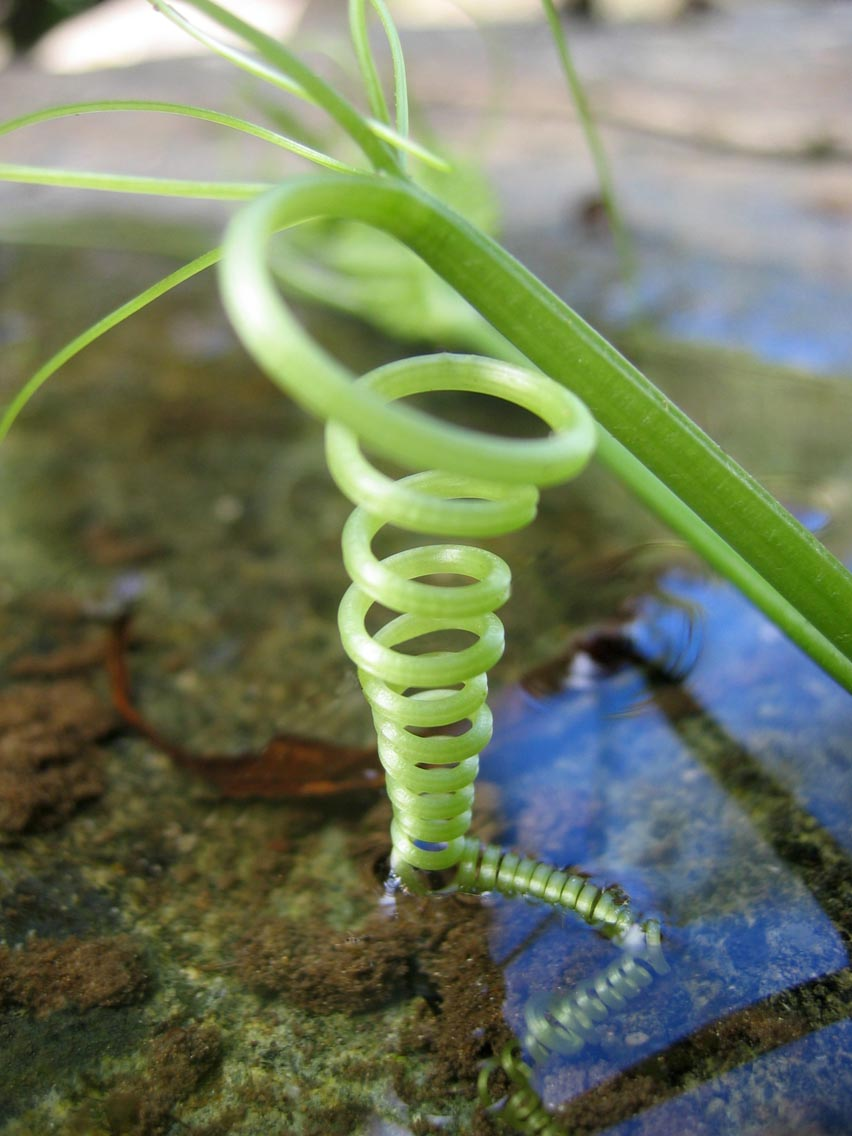
\includegraphics[scale=0.2]{figuras/DirkvdM_natural_spiral.jpg}
\end{minipage}
\begin{minipage}{0.35\textwidth}
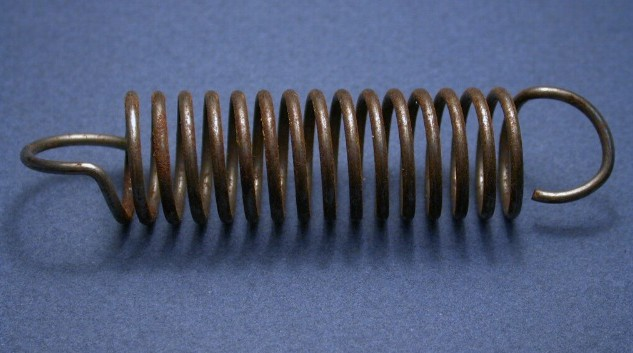
\includegraphics[scale=1]{figuras/mola.jpg}
\end{minipage}
\begin{minipage}{0.33\textwidth}

\includegraphics[scale=1]{figuras/introducao/dna.png}
\end{minipage}

\newpage

\marcador{subsection}{Parametrização por inteseção de superfícies}


\begin{itemize}
\item {\color{red}NÃO} existe equação cartesiana de curvas em {\color{red}\(\R^3\)};

\item Uma equação cartesiana no {\color{red}\(\R^3\)} {\color{red}SEMPRE} representa uma superfície.

\begin{center}
{\color{blue}\(y+z=2\) é um plano} e
{\color{orange}\(x^2+y^2=1\) é um cilindro.}
\end{center}
\end{itemize}

Muitas curvas no espaço, podem ser parametrizadas via interseção de duas superfícies.

\begin{center}
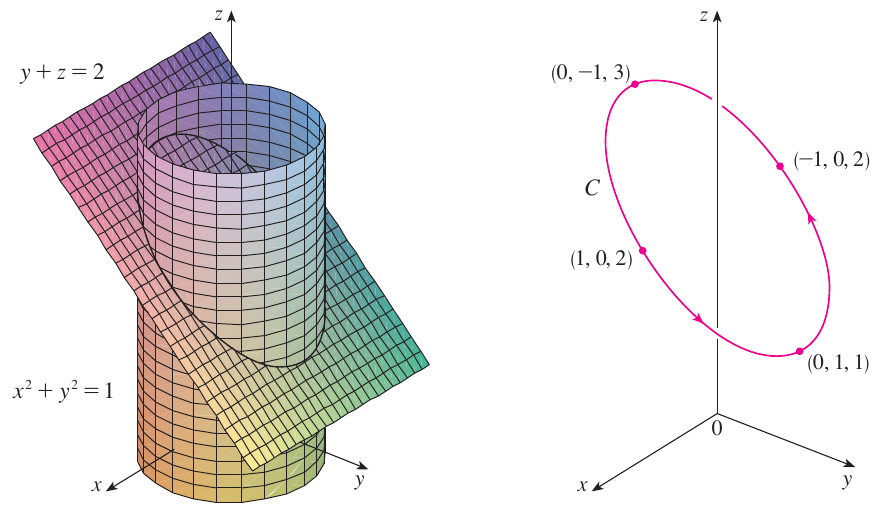
\includegraphics[scale=0.7]{figuras/curvas/cilindro-plano.png}
\end{center}

\begin{exeb}{}{}
 Determine uma equação vetorial que represente a curva obtida pela interseção das superfícies:
\begin{enumerate}
\item Os planos: \(y+z=1\) e \(x+y=1\);

\item O cone \(z=\sqrt{x^2+y^2}\) e o plano \(x+y=1\);

\item  da esfera $x^2+y^2+z^2-2z=3$ com o plano $z=\frac{3}{2}$;

\item do cilindro $x^2+y^2=1$ com o plano $y+z=2$;

\item do paraboloide $x^2+y+z^2=1$ com o cilindro $y=x^2$.

%\item  da esfera $x^2+y^2+z^2=1$ com o cilindro $y=x^2$.
\end{enumerate}
\end{exeb}
